\documentclass[10pt,a4paper]{article}
\usepackage[a4paper, total={6.5in, 9in}]{geometry}
\usepackage[latin1]{inputenc}
\usepackage{amsmath}
\usepackage{amsfonts}
\usepackage{amssymb}
\usepackage{mathtools}
\usepackage{graphicx}
\usepackage{float}
\usepackage[usenames, dvipsnames]{color}
\usepackage{fancyhdr}
\usepackage{enumitem}
\usepackage{listings}
\setlength{\headheight}{15.2pt}
\pagestyle{fancy}
\setlength{\parindent}{0em}
\setlength{\parskip}{10pt}
\setlist[enumerate,1]{label=\alph*)}
\setlist[enumerate,2]{label=(\roman*)}
\definecolor{LGray}{gray}{0.9}
\lstset{language=python, tabsize=2, breaklines=true, postbreak=\mbox{\textcolor{red}{$\hookrightarrow$}\space}, basicstyle=\linespread{0.7}\ttfamily, } 
\newcommand*\diff{\mathop{}\!\mathrm{d}}



\begin{document}
\title{ENGSCI763 A1}
\author{Benjamin Yi}
\rhead{Benjamin Yi - byi649 - 925302651}
\lhead{ENGSCI763 A1}
	
\section*{Question 1}
\begin{align*}
	P(Z=z) &= P(X + Y = z) \\
	&= \sum_{i=0}^{z}P(X + Y = z, X = i) \\
	&= \sum_{i=0}^{z}P(Y = z - i, X = i) \\
	&= \sum_{i=0}^{z}P(Y = z - i) \times P(X = i) \\
	&= \sum_{i=0}^{z}\bigg[\frac{\mu^{(z-i)}e^{-\mu}}{(z-i)!}\bigg]\times\bigg[\frac{\lambda^ie^{-\lambda}}{i!}\bigg]\\
	&= \sum_{i=0}^{z}\frac{e^{-(\mu + \lambda)}\mu^{(z-i)}\lambda^i}{(z-i)!\times i!}\\
	&= \sum_{i=0}^{z}\frac{1}{z!}\times\frac{z!}{(z-i)!\times i!}\times e^{-(\mu + \lambda)}\mu^{(z-i)}\lambda^i\\
	&= \sum_{i=0}^{z}\bigg[\frac{z!}{(z-i!)\times i!} \times \lambda^i \times \mu^{(z-i)}\bigg] \times \frac{e^{-(\mu + \lambda)}}{z!}\\
	&= \sum_{i=0}^{z} \bigg[{z \choose i} \times \lambda^i \times \mu^{(z-i)}\bigg] \times \frac{e^{-(\mu + \lambda)}}{z!}\\
	&= (\lambda + \mu)^z \times \frac{e^{-(\mu + \lambda)}}{z!}\\
\end{align*}
The last step appears from recognizing the binomial theorem. The final expression is the equation for a Poisson process with rate = \((\lambda + \mu)\), therefore \(Z(t)\) is also a Poisson process.

\newpage
\section*{Question 2}
\begin{figure}[H]
	\centering
	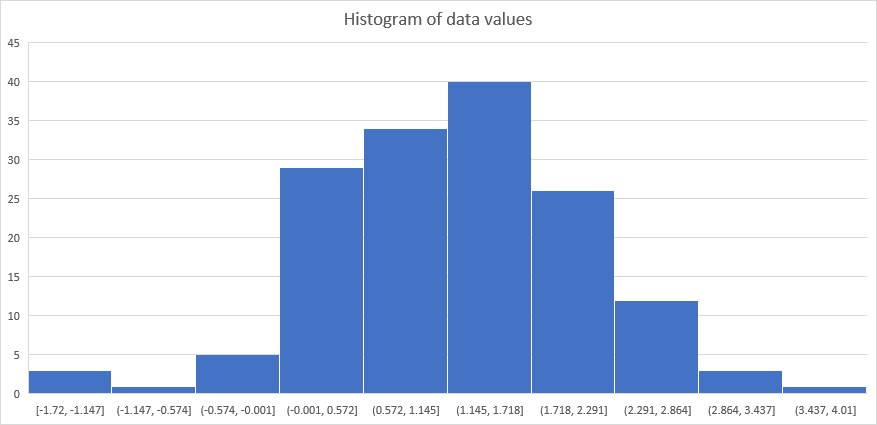
\includegraphics[width=0.7\linewidth]{q2hist}
\end{figure}
Looking at the histogram of the data with number of bins = 10, I hypothesised a normal distribution for the data, with the first and last bin extended to positive and negative infinity. Using Maximum Likelihood Estimators to estimate the two parameters of a normal distribution:

\begin{align*}
	f(x) &= \frac{1}{\sqrt{2\pi\sigma^2}} \times \text{exp}\bigg(-\frac{(x-\mu)^2}{2\sigma^2}\bigg)\\
	L(\mu, \sigma^2) &= \prod_{i=0}^{j} \frac{1}{\sqrt{2\pi\sigma^2}} \times \text{exp}\bigg(-\frac{(x_i-\mu)^2}{2\sigma^2}\bigg)\\
	&= \bigg(\frac{1}{\sqrt{2\pi\sigma^2}}\bigg)^n \times \prod_{i=0}^{j} \text{exp}\bigg(-\frac{(x_i-\mu)^2}{2\sigma^2}\bigg)\\
	&= \bigg(\frac{1}{\sqrt{2\pi\sigma^2}}\bigg)^n \times \text{exp}\bigg(-\frac{1}{2\sigma^2}\sum_{i=0}^{n}(x_i-\mu)^2\bigg)\\
\end{align*}

Using log maximum likelihood:

\begin{align*}
	l(\mu, \sigma^2) &= \ln (L(\mu, \sigma^2)) \\
	&= \ln \bigg(\bigg(\frac{1}{\sqrt{2\pi\sigma^2}}\bigg)^n\bigg) + \ln \bigg(\text{exp}\bigg(-\frac{1}{2\sigma^2}\sum_{i=0}^{n}(x_i-\mu)^2\bigg) \\
	&= -\frac{n}{2} \ln (2\pi\sigma^2) - \frac{1}{2\sigma^2}\sum_{i=0}^{n}(x_i - \mu)^2 \\
	&= -\frac{n}{2} \ln (2\pi) - \frac{n}{2} \ln (\sigma^2) - \frac{1}{2\sigma^2}\sum_{i=0}^{n}(x_i - \mu)^2 \\
\end{align*}

Differentiating and setting to zero to find parameters:

\begin{align*}
	\frac{\partial l}{\partial \mu} &= \frac{1}{\sigma^2} \sum_{i=0}^{n}(x_i-\mu)^2\\
	0 &= \sum_{i=0}^{n}(x_i-\mu)^2\\
	0 &= \sum_{i=0}^{n}(x_i)- n\mu\\
	\mu &= \frac{\sum_{i=0}^{n}x_i}{n}
\end{align*}

\begin{align*}
	\frac{\partial l}{\partial \sigma^2} &= -\frac{n}{2\sigma^2} + \frac{1}{2\sigma^4} \sum_{i=0}^{n}(x_i-\mu)^2\\
	&= \frac{1}{2\sigma^2}\bigg[\frac{1}{\sigma^2}\sum_{i=0}^{n}(x_i-\mu)^2 - n\bigg]\\
	0 &= \frac{1}{\sigma^2}\sum_{i=0}^{n}(x_i-\mu)^2 - n \\
	\sigma^2 &= \frac{\sum_{i=0}^{n}(x_i-\mu)^2}{n}\\
\end{align*}

Therefore the maximum likelihood parameters are the sample mean and sample variance.

Using the ten bins as shown previous, a \(\chi^2\) test was performed to evaluate goodness of fit.
\begin{table} [H]
	\centering
	\begin{tabular}{c|c|c|c|c} 
		Bin	&  Range & Estimated n & Actual n & \(\chi^2\)\\ 
		\hline 
		1	&  -inf, -1.147 & 0.753 & 3 & 6.71\\  
		2	&  -1.147, -0.574 & 3.09 & 1 & 1.41\\ 
		3	&  -0.574, -0.001 & 10.1 & 5 & 2.56\\ 
		4	&  -0.001, 0.572 & 22.6 & 29 & 1.81\\ 
		5	&  0.572, 1.145 & 34.8 & 34 & 0.0177\\ 
		6	&  1.145, 1.718 & 36.8 & 40 & 0.281\\ 
		7	&  1.718, 2.291 & 26.7 & 26 & 0.0198\\ 
		8	&  2.291, 2.864 & 13.3 & 12 & 0.134\\ 
		9	&  2.864, 3.437 & 4.57 & 3 & 0.540\\ 
		10	&  3.437, +inf & 1.27 & 1 & 0.0571\\ 
	\end{tabular} 
\end{table}

\(\chi^2\) sums to 13.54, which is lower than the value 16.92 needed for a 95\% confidence with 9 degrees of freedom - therefore we accept the null hypothesis and are satisfied with goodness of fit with normal distribution with mean = 1.23 and variance = 0.847.

\newpage
\section*{Question 3}
The random observations were generated in python, with the following code: \\
\lstinputlisting{generate.py}

\begin{figure}[H]
	\centering
	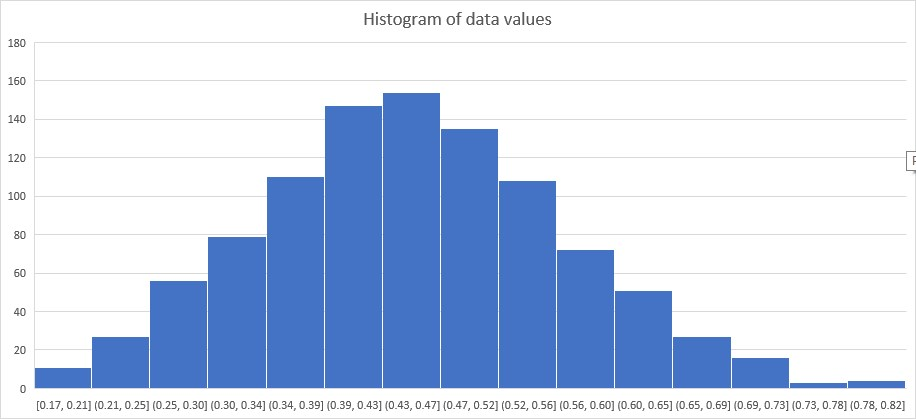
\includegraphics[width=0.7\linewidth]{q3hist}
\end{figure}
Looking at the histogram of the data with number of bins = 15, I hypothesised a beta distribution for the data. Matching moments to estimate the two parameters of a beta distribution:

\begin{align*}
	\mu &= \frac{\alpha}{\alpha + \beta}\\
	\alpha &= \mu(\alpha + \beta)\\
	\beta &= \frac{\alpha(1-\mu)}{\mu}
\end{align*}

\begin{align*}
	\sigma^2 &= \frac{\alpha\beta}{(\alpha+\beta)^2(\alpha+\beta+1)}\\
	&=\alpha^2\mu^2(1-\mu)\bigg/\bigg[\mu^2\bigg(\alpha + \frac{\alpha(1-\mu)}{\mu}\bigg)^2 \times \mu\bigg(\alpha + \frac{\alpha(1-\mu)}{\mu} + 1\bigg)\bigg]\\
	&=\alpha^2\mu^2(1-\mu)\bigg/\bigg[\bigg(\alpha\mu + \alpha(1-\mu)\bigg)^2 \times \bigg(\alpha\mu + \alpha(1-\mu) + \mu\bigg)\bigg]\\
	&=\alpha^2\mu^2(1-\mu)\bigg/\bigg[\alpha^2(\alpha+\mu)\bigg]\\	
	&= \frac{\mu^2(1-\mu)}{(\alpha+\mu)}
\end{align*}

Re-arrange to give:

\begin{align*}
	\alpha &= \frac{\mu^2(1-\mu)}{\sigma^2} - \mu\\
	\beta &= \frac{\alpha(1-\mu)}{\mu}
\end{align*}

Using 15 bins\footnote{Not as in figure, because Excel does not allow fine grain tuning of histogram bins} , a \(\chi^2\) test was performed to evaluate goodness of fit.
\begin{table} [H]
	\centering
	\begin{tabular}{c|c|c|c|c} 
		Bin	&  Range & Estimated n & Actual n & \(\chi^2\)\\ 
		\hline 
		1	&  0, 1/15 & 0.00354 & 0 & 0.00354\\  
		2	&  1/15, 2/15 & 0.585 & 0 & 0.585\\ 
		3	&  2/15, 3/15 & 8.31 & 7 & 0.208\\ 
		4	&  3/15, 4/15 & 40.5 & 42 & 0.0580\\ 
		5	&  4/15, 5/15 & 106 & 107 & 0.0133\\ 
		6	&  5/15, 6/15 & 181 & 170 & 0.636\\ 
		7	&  6/15, 7/15 & 221 & 239 & 1.42\\ 
		8	&  7/15, 8/15 & 202 & 194 & 0.347\\ 
		9	&  8/15, 9/15 & 139 & 137 & 0.0368\\ 
		10	&  9/15, 10/15 & 70.5 & 70 & 0.00344\\ 
		11	&  10/15, 11/15 & 24.7 & 27 & 0.207\\ 
		12	&  11/15, 12/15 & 5.35 & 5 & 0.0224\\ 
		13	&  12/15, 13/15 & 0.561 & 2 & 3.69\\ 
		14	&  13/15, 14/15 & 0.0168 & 0 & 0.0168\\ 
		15	&  14/15, 15/15 & 0.0000269 & 0 & 0.0000269\\ 
	\end{tabular} 
\end{table}

\(\chi^2\) sums to 7.24, which is lower than the value 23.68 needed for a 95\% confidence with 14 degrees of freedom - therefore we accept the null hypothesis and are satisfied with goodness of fit with beta distribution with \(\alpha = 8.21\) and \(\beta = 9.98\).

\newpage
\section*{Question 4}
\begin{align*}
	f(x) &= (1-p)^{x-1}p\\
	L(p) &= \prod_{i=1}^{n}(1-p)^{x_i-1}p\\
	&= p^n\prod_{i=1}^{n}(1-p)^{x_i-1}\\
	&= \frac{p^n}{(1-p)^n}\prod_{i=1}^{n}(1-p)^{x_i}
\end{align*}

\begin{align*}
	l(p) &= \ln L(p)\\
	&= \ln \bigg(\frac{p^n}{(1-p)^n}\bigg) + \sum_{i=0}^{n}\ln\bigg[(1-p)^{x_i}\bigg]\\
	&= n \ln \bigg(\frac{p}{1-p}\bigg) + \sum_{i=0}^{n}x_i\ln(1-p)\\
	&= n \ln (p) - n\ln(1-p) + \sum_{i=0}^{n}x_i\ln(1-p)\\
	&= n \ln (p) + \bigg[\sum_{i=0}^{n}x_i - n\bigg]\ln(1-p)\\
\end{align*}

Differentiating and setting to zero to find parameter:

\begin{align*}
	\frac{dl}{dp} &= \frac{n}{p} + \bigg[\sum_{i=0}^{n}x_i - n\bigg]\frac{1}{1-p}\\
	0 &= n(1-p) + \bigg[\sum_{i=0}^{n}x_i - n\bigg]p\\
	0 &= n - np + \bigg[\sum_{i=0}^{n}x_i - n\bigg]p\\
	0 &= p\bigg(\bigg[\sum_{i=0}^{n}x_i - n\bigg] - n\bigg) + n\\
	p &= -n \bigg/ \bigg(\bigg[\sum_{i=0}^{n}x_i - n\bigg] - n\bigg)\\
	&= \frac{n}{\sum_{i=0}^{n}x_i}\\
	&= \frac{1}{\mu}
\end{align*}

The maximum likelihood estimator for p is the reciprocal of the mean.

This estimator is not unbiased. To be unbiased, \(E[\hat{p}] = p\) for all n. Consider n = 1:

\begin{align*}
	E\bigg[\frac{1}{X_1}\bigg] &= \sum_{x=1}^{\infty}\frac{1}{x}P(X_1 = x)\\
	&= \sum_{x=1}^{\infty}\frac{1}{x}(1-p)^{x-1}p\\
	&= p + \sum_{x=2}^{\infty}\frac{1}{x}(1-p)^{x-1} \, \, \, > p\\
\end{align*}

The condition is not met so the estimator is biased.

\newpage
\section*{Question 5}
\begin{enumerate}
\item
The variances were found using python, with the following code:\\
\lstinputlisting{mc.py}

Variance under iid and under antithetic sampling were very similar (0.01009 vs 0.00944 respectively). Therefore antithetic sampling is neutral for the example.

\item
Antithetic sampling is useful when the problem is mostly odd, as it removes the odd part of the variance and doubles the even part of the variance. Because antithetic sampling was neutral for this example, it means the problem was equally even and odd (or close enough that the simulation could not find a difference in 1000 runs).
\end{enumerate}
\newpage
\section*{Question 6}
\begin{enumerate}
\item
It is clear that to maintain feasibility and minimise cost, x must equal 0.5 for the first stage. Then:

\begin{equation*}
	y = 
		\begin{cases}
			\omega - x & \text{if } \omega \geq x \text{  with }  p=\frac{2}{3} \\
			0 & \text{otherwise} \text{  with } p=\frac{1}{3} \\
		\end{cases}
\end{equation*}

\begin{align*}
	E[z] &= 5 \times 0.5 + \bigg(E[\omega | \omega \geq x] - 0.5\bigg)\bigg(\frac{2}{3}\bigg) + 0 \times\bigg(\frac{1}{3}\bigg)\\
	&= 2.5 + \bigg(1-0.5\bigg)\bigg(\frac{2}{3}\bigg)\\
	&= 2.83
\end{align*}

The expected cost is 2.83 \\

\item 
\begin{align*}
	E[\omega] &= 0.75 \\
	x &= 0 \\
	y &= \omega
\end{align*}

\begin{align*}
E[z] &= 0 + E[\omega | \omega \leq 1]\bigg(\frac{2}{3}\bigg) + \infty \times\bigg(\frac{1}{3}\bigg)\\
&= \infty
\end{align*}

The infinity arises due to potential infeasibility as in stage one, we set x = 0. Then in stage 2, there is a 1/3 chance \(\omega\) takes upon a value greater than 1, and the constraints cannot be met. This gives a cost of infinity.

\item 
As the cost of expected value problem is infinity, the VSS is also infinity (\(\infty - 2.83 = \infty\)).

\end{enumerate}

\end{document}

